\begin{figure}[tbp]
\centering
\sporkCodeRule
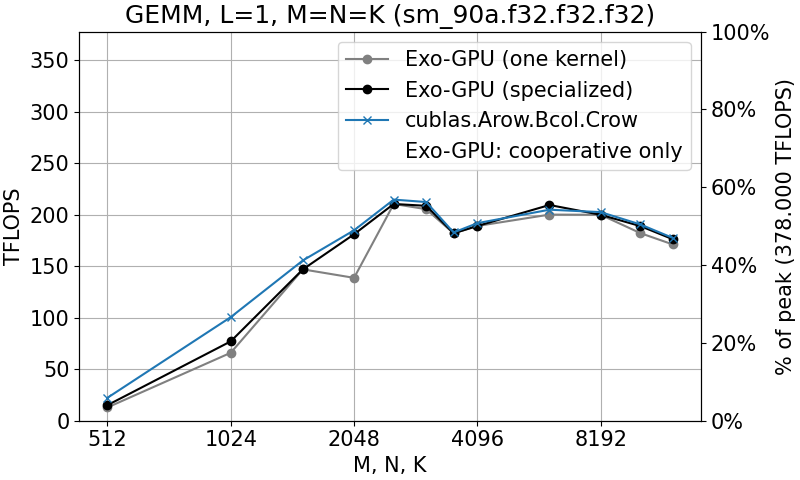
\includegraphics[width=0.45\linewidth]{data-2026-11-11/out_plot/f32_coop/L1_square_sm_90a_f32_f32.png}
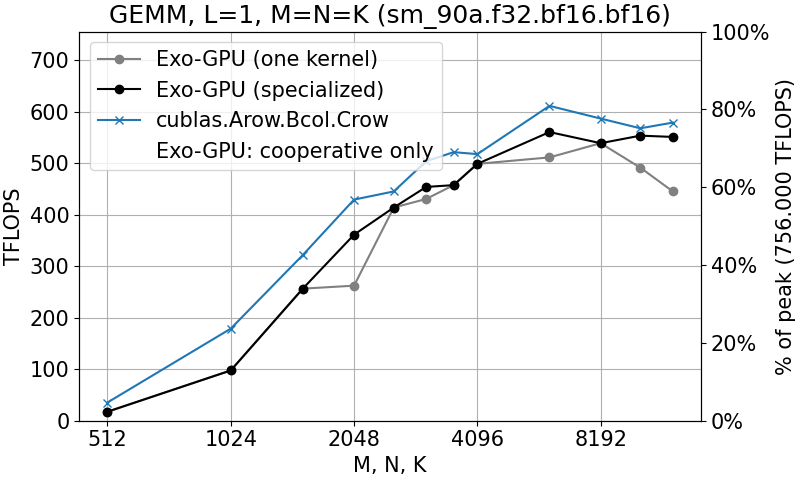
\includegraphics[width=0.45\linewidth]{data-2026-11-11/out_plot/bf16_coop/L1_square_sm_90a_f32_bf16.png}

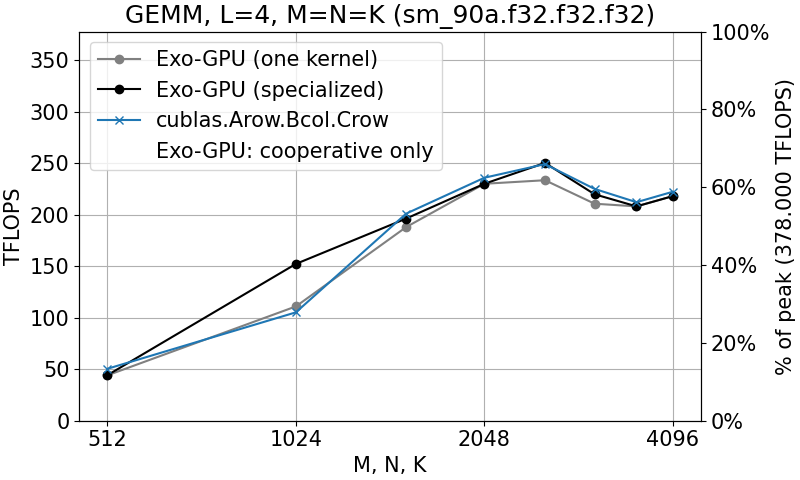
\includegraphics[width=0.45\linewidth]{data-2026-11-11/out_plot/f32_coop/L4_square_sm_90a_f32_f32.png}
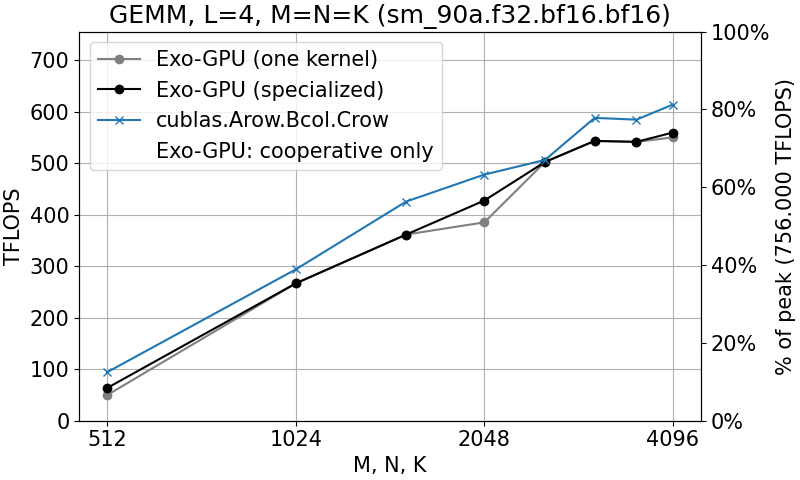
\includegraphics[width=0.45\linewidth]{data-2026-11-11/out_plot/bf16_coop/L4_square_sm_90a_f32_bf16.png}

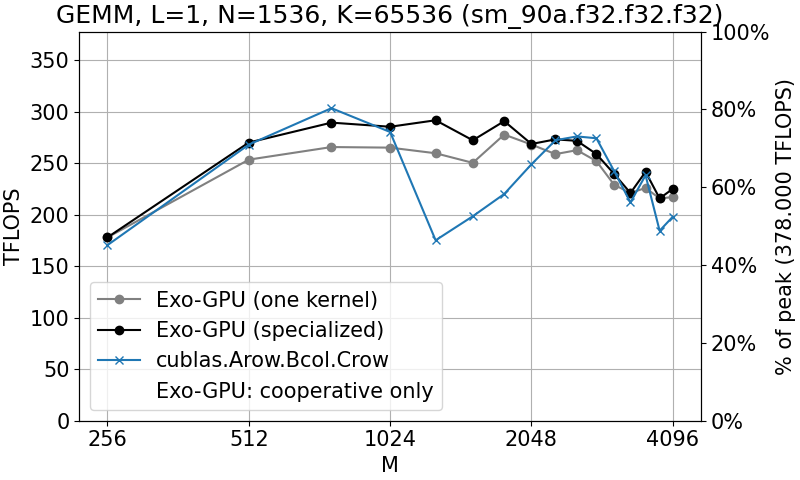
\includegraphics[width=0.45\linewidth]{data-2026-11-11/out_plot/f32_coop/L1K65536_sm_90a_f32_f32.png}
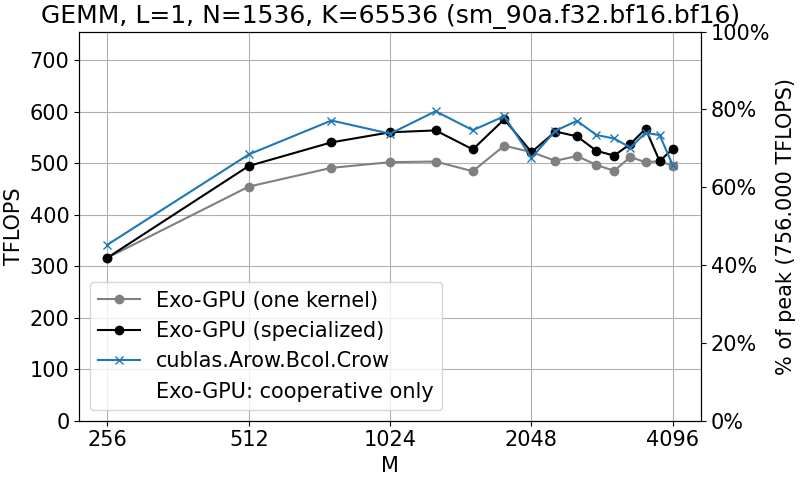
\includegraphics[width=0.45\linewidth]{data-2026-11-11/out_plot/bf16_coop/L1K65536_sm_90a_f32_bf16.png}

\caption{Comparison between \sporkName{} \texttt{sm\_90a} cooperative gemm kernels and CUBLAS,
with both tf32 (left) and bf16 (right) input precision;
the former requires CUBLAS to be set with math mode \texttt{CUBLAS\_TF32\_TENSOR\_OP\_MATH}
and has half the theoretical peak FLOPS.
The bottom row shows \texttt{K=65536} problem sizes,
which non-trivially exercise the split-K optimization.
\texttt{L} is the batch size.}
\label{fig:Sm90aCoopPlots}
\sporkCodeRule
\end{figure}
